\documentclass{article}
\newcommand\hmmax{0}
\newcommand\bmmax{0}
\usepackage{booktabs}

%% Language and font encodings
\usepackage[english]{babel}
\usepackage[utf8x]{inputenc}
\usepackage[T1]{fontenc}
\usepackage{gensymb}
\usepackage{pdfpages}
\usepackage{mparhack}


\usepackage[bitstream-charter]{mathdesign}
\let\circledS\undefined
%% Sets page size and margins
\usepackage[a4paper,top=2cm,bottom=2cm,left=1cm,right=1cm, marginparsep=1cm]{geometry}

%% Useful packages
\usepackage{amsmath}
\usepackage{bm}
\usepackage[makeroom]{cancel}
\usepackage{enumitem}
\usepackage{listings}
\usepackage{multirow}
\usepackage{amssymb}
\usepackage{float}
\usepackage{graphicx}
\usepackage[colorinlistoftodos]{todonotes}
\usepackage[colorlinks=true, allcolors=blue]{hyperref}
\usepackage[final]{matlab-prettifier}
\usepackage{courier}
\usepackage{algorithm}
\usepackage[noend]{algpseudocode}
\usepackage[]{appendix}
\usepackage{wrapfig}
\usepackage[final]{matlab-prettifier}
\usepackage[final]{mathtools}

\renewcommand\labelitemi{$\bullet$}

\definecolor{codecol}{rgb}{0.94, 0.94, 0.94}
\definecolor{dgreen}{rgb}{0.1, 0.49, 0.1}

\newcommand{\ea}{\nonumber \\}
\lstset{basicstyle=\footnotesize\ttfamily,breaklines=true}
\lstset{framextopmargin=50pt,frame=bottomline}

\newcommand{\norm}[2]{\left\Vert#1\right\Vert_{#2}}
\newcommand{\question}[1]{{\color{red}\textbf{Question: }\emph{#1}}}
\newcommand{\action}[1]{{\color{blue}\textbf{Action: }\emph{#1}}}
\newcommand{\epdp}{$(\epsilon, \delta)$-DP}
\newcommand{\alg}{$\mathcal{A}$}
\newcommand{\data}{$\mathcal{D}$}
\newcommand{\vect}[1]{\boldsymbol{\mathbf{#1}}}
\newcommand{\normaldist}[2]{$\mathcal{N}(#1, #2)$}
\newcommand{\expt}[2]{\mathbb{E}_{#2}[#1]}
\newcommand{\prob}[2]{\mathbb{P}_{#2}[#1]}
\newcommand{\model}[1]{\mathcal{M}_{#1}}
\newcommand{\indep}{\raisebox{0.05em}{\rotatebox[origin=c]{90}{$\models$}}}
\newcommand{\mset}[3]{\lbrace {#1}_{#2} \rbrace_{#2=1}^{#3} }
\DeclarePairedDelimiter{\ceil}{\lceil}{\rceil}
\DeclarePairedDelimiter\floor{\lfloor}{\rfloor}

\newcommand{\ix}[1]{%
  \leavevmode % if at the start of a paragraph
  \marginpar{\small\emph{#1}}% the note
}

\newcommand{\qx}[1]{%
	\leavevmode % if at the start of a paragraph
	\marginpar{\color{blue}\small\emph{#1}}% the note
}
\newcommand{\marfig}[2]{
  \marginpar{ \includegraphics[width=\marginparwidth]{#1} \centering \text{\small #2} }
}

\newcommand{\myq}[1]{%
	\vspace{1em}
	\noindent\underline{\emph{Exercise #1}}\vspace{0.25em}\linebreak
}

\DeclareMathAlphabet{\altmathcal}{OMS}{cmsy}{m}{n}

\title{\textbf{Reinforcement Learning: An Introduction}\\
\textit{Solutions: Chapter 2}
}
\author{Mrinank Sharma}

\begin{document}
\maketitle

\myq{2.1 $\epsilon$-Greedy Action Selection}
\begin{align}
\text{Pr}[\text{greedy action selected}] &= \epsilon \cdot \frac{1}{2} + (1 - \epsilon) \\
&= \frac{3}{4}
\end{align}

\myq{2.2 Bandit Example}
The exploratory action could have occured on any of the timesteps (and the behaviour could have coincidently given us the sequence of actions). However, the action \textbf{must} have occured on timesteps $2$ and $5$ since the greedy action was not selected. 

\myq{2.3 Infinite Horizon Performance}
In the long run, assume that the sample averages have converged to the correct values or close enough for the exploratory cases. There is no guarantee of this happenign for the purely greedy strategy. Then, the probability of selecting the right action is $0.99$ and $0.9$ for $\epsilon=0.01$ and $\epsilon=0.1$ respectively and from the graph, about $\frac{1}{3}$ for the purely greedy example. 

The greedy algorithm seems to average about $1$ reward on each timestep (I'm sure there are mathematical reasons for this). So, in the long run, it would have cumulative reward $T$. The \emph{expected value} of a purely exploratory action is $0$, since the arm means are drawn from a $\altmathcal{N}(0, 1)$ distribution. As a result, in the long run:
\begin{align}
\text{expected cumulative reward}_{\epsilon=0.01} &= 0.99 \cdot 1.55\cdot T\\
\text{expected cumulative reward}_{\epsilon=0.1} &= 0.9 \cdot 1.55\cdot T 
\end{align}

\myq{2.4 Changing Step Sizes}
Note: might have got the indices slightly confused here!
\begin{align}
Q_{n+1} &= Q_n + \alpha_n\ [R_n - Q_n] \nonumber\\ 
&= \alpha_n R_n + (1-\alpha_n) Q_n \nonumber \\
&= \alpha_n R_n +  (1-\alpha_n) \alpha_{n-1} R_{n-1} + (1-\alpha_n)  (1-\alpha_{n-1}) Q_{n-1} \nonumber\\
& \vdots \nonumber \\
& = \sum_{i=0}^{n-1} \alpha_{n-i} R_{n-i} \prod_{j=0}^{i-1} (1 - \alpha_{n-j}) + Q_1 \prod_{i=0}^{n-1} (1-\alpha_{n-1})
\end{align}

\myq{2.5 Programming}
\begin{figure}[H]
	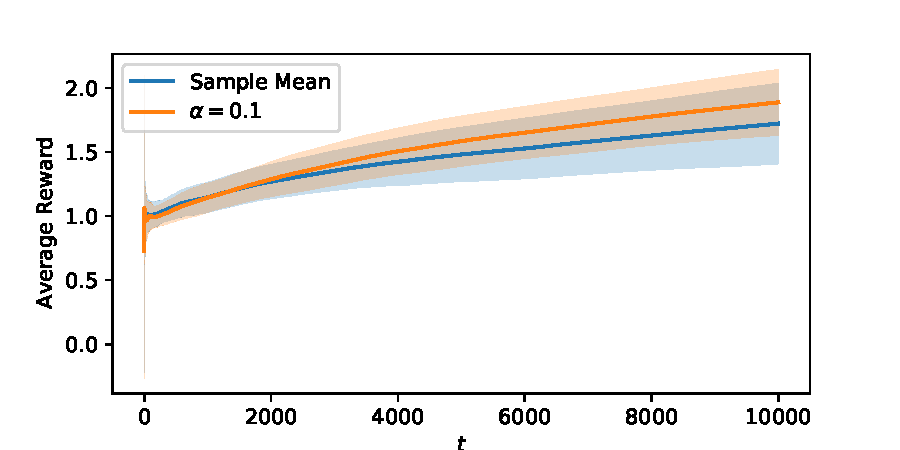
\includegraphics{rewards.pdf}
	\centering
\end{figure}

\begin{figure}[H]
	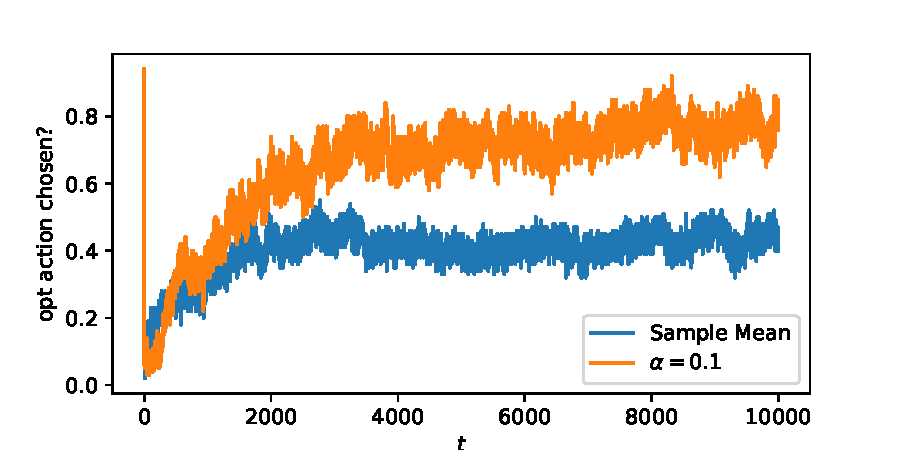
\includegraphics{choices.pdf}
	\centering
\end{figure}

As expected, the sample mean method does not work so well. I expect it to get worse as more time goes on, but it still seems to do reasonably well. 

\myq{2.6 Mysterious Spikes}
The spikes only occur for the optimistic, greedy method even though we've averaged across $2000$ different bandit problems. 

The algorithm has wildly too high initial values. This effectively means that for the first ten steps, the algorithm will explore every single option. After the $10$th step, the algorithm will greedily pick the best option. This is most likely to be the true best option. However, eventually it will pick this option enough times that it no longer looks like the true best option (since the other estimates values are all too high). It will then pick those options until their value drops, and this keeps repeating. 

This sort of behaviour won't get smoother as we randomise more. We are always dealings with updates from small numbers of rewards with poor initial values and as a result, the estimated value for each of the arms will be changing most at the start, meaning that there will be oscillations in the optimal action selected. 

\textbf{I'm not particularly convinced by this answer. }

\myq{2.7: Unbiased Constant Step Size Trick}
Since $\bar{o}_0 = 0 $, $\bar{o}_1 = \alpha$ so it is clear that $Q_2 = R_1$. Therefore, there is no initial bias. 

We need to show that the remaining terms form an weighted average. Let's go back to our previous formula. Doing some relabeling, we can write $Q_{n+1}$ as:

\begin{align}
Q_{n+1} = \sum_{i=1}^n R_i \beta_i \prod_{j=i+1}^n  (1- \beta_j).
\end{align}
We want to show that the coefficients form a weighted average. It is easy to see that:
\begin{align}
\beta_i = \frac{1}{\sum_{j=0}^{i-1} (1-\alpha)^j}.
\end{align}
$\beta_i > 0\ \forall i$ and $\beta_i > \beta_{i+1}$. We want to show that:
\begin{align}
\sum_{i=1}^n \beta_i \prod_{j=i+1}^n  (1- \beta_j) = 1.
\end{align}
We now show that the coefficients sum to $1$ by proof by induction. Consider the case $n=1$.  Clearly the coefficients sum to $1$, since $\beta_1 = 1$. Now, assume that the above holds for $n=n^*$. Then,

\begin{align}
\sum_{i=1}^{n^* + 1} \beta_i \prod_{j=i+1}^{n^* + 1}  (1- \beta_j) = \beta_{n^*+1} + (1-\beta_{n^*+1}) \underbrace{\sum_{i=1}^{n^*} \beta_i \prod_{j=i+1}^{n^*}  (1- \beta_j)}_{1} = 1
\end{align} 
If true for $n$, true for $n+1$. Since true for $n=1$, true for all positive integers. Thus we have a exponentially weighted average with no initial bias.  

\myq{2.8: UCB Spikes}
The algorithm will explore every single action first because all of the arm counts are zero. On the $11$th step, it will pick what seems to be the best option \textbf{across all of the games}, giving the spike in most cases (depending on the exact draws, not always the best value), but then the uncertainty reward will go down, leading to other arms being picked. 

If $c=1$ is used, the spike is less prominent as the reward for uncertainty is smaller. The algorithm requires more draws from the best arm to sample other arms, giving a smoother curve. The larger the value of $c$, the more quickly the estimates are likely to be changing (due to large changes in the uncertainty), so the noisier the curves. 

\myq{2.9: Softmax}
Suppose $a \in \lbrace 0, 1\rbrace$. Then:
\begin{align}
\text{Pr}(A_t = 0) &= \frac{\exp H_t(0)}{\exp(H_t(0)) + \exp(H_t(1))} \nonumber \\
&= \frac{1}{1 + \exp(-(H_t(0) - H_t(1)))},
\end{align}
Which looks just like the sigmoid function:
\begin{align}
\sigma(z) = \frac{1}{1 + \exp(-z)},
\end{align}
with $z =H_t(0) - H_t(1)$ 

\myq{2.10: Contextual Bandits}
If we do not know which case we are in, we pick the action with the maximum expected reward. However, in this case, it is $0.5$ for both actions, marginalised across the cases. The best we can expect to do is to choose arbitarily, receiving average reward $0.5$. 

Alternatively, if we are informed which case we are in, we can solve this problem by treating it as two seperate bandit problems and applying a typical bandit algorithm, such as UCB. 

\myq{2.11: Non-Stationary Comparison}
Please see the below figure.

\begin{figure}[H]
	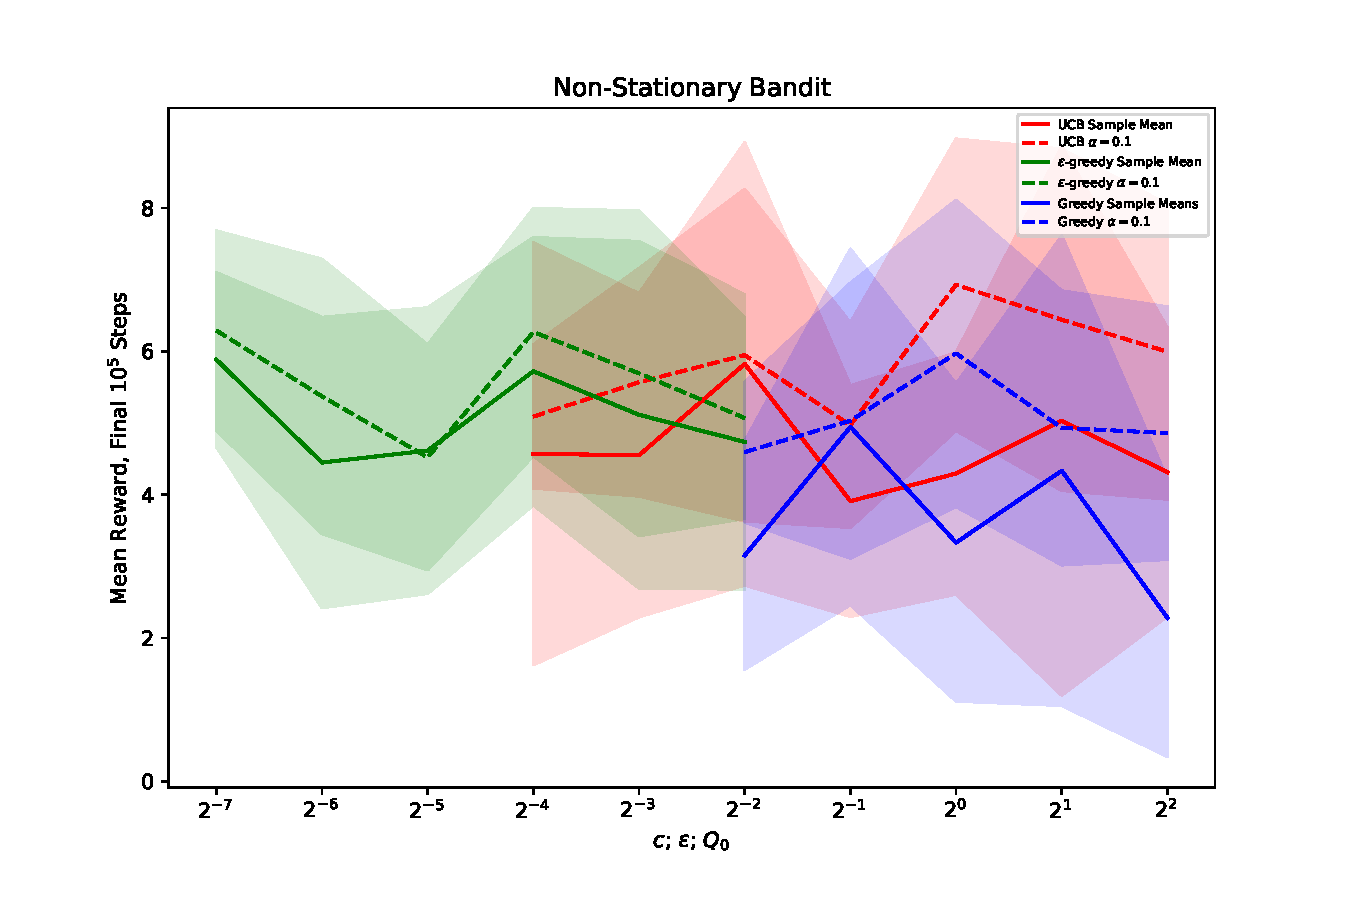
\includegraphics[width=\textwidth]{comparison.pdf}
	\centering
\end{figure}
As expected, the sample average performs worse than the constant step size update. This pattern can consisently be seen. 

The graphs are \emph{very} noisy, perhaps because we have only chosen ten seeds. It would have probably been better to fix the bandit problem (or series of bandit problems) - that could itself be a large cause of the noise. 

Despire this, the greedy method with an optimistic initialisation does poorly. The exploration is encouraged only at the start, but the method should keep exploring throughout the entire sequence, which will not be happening. It is suprising that UCB does as well as it does especially since the notion of uncertainty is now basically incorrect. It would seem that large values of $c$, which encourage more exploration, seem to do better using a step size. 

\textbf{If I were to do this again, I would run this with a series of fixed bandit problems i.e., fix the random walk which the bandits go on. This would reduce the variance in the graph and hopefully make it easier to spot patterns. } 

\end{document}